%% LaTeX2e class for student theses
%% sections/apendix.tex
%% 
%% Karlsruhe Institute of Technology
%% Institute for Program Structures and Data Organization
%% Chair for Software Design and Quality (SDQ)
%%
%% Dr.-Ing. Erik Burger
%% burger@kit.edu
%%
%% Version 1.3.5, 2020-06-26

\chapter{Acknowledgements}
I would like to thank Prof. Dr. Stamatakis and Lukas Hübner for their enlightening advice throughout the last four months, my parents for their continued support throughout my studies, and Katrin Anne Mertes and Max Lennart Steiert for proofreading this thesis.
\\

This work was performed on the computational resource bwUniCluster funded by the Ministry of Science, Research and the Arts Baden-Württemberg and the Universities of the State of Baden-Württemberg, Germany, within the framework program bwHPC.
This project has received funding from the European Research Council (ERC) under the European Union’s Horizon 2020 research and innovation program (grant agreement No. 882500).
\\
\vspace{4cm}

\includegraphics[scale=0.1]{logos/erc.png}

%\chapter{Glossary}
\printglossary[type=\acronymtype]
\printglossary

\iflanguage{english}
{\chapter{Appendix}}    % english style
{\chapter{Anhang}}      % german style
\label{chap:appendix}

\section{Buffer Subtree-Flushing Criterion Comparison}

\begin{figure}[h!]
\centering
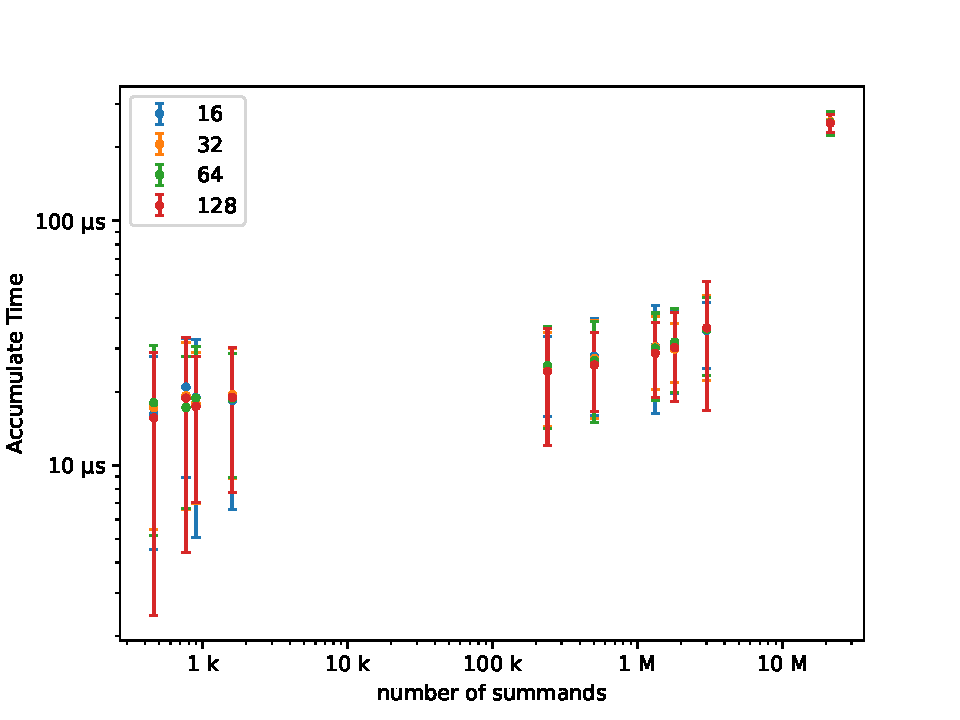
\includegraphics[scale=0.8]{figures/bufferSizes.pdf}
\caption{Accumulation runtime with different subtree sizes used as flushing criterion.}
\label{fig:bufferFlushingCriterion}
\end{figure}

\section{Detailed Benchmark Results}
\,
\newcommand{\mScale}{0.72}

\begin{figure}
\begin{subfigure}{\textwidth}
\centering
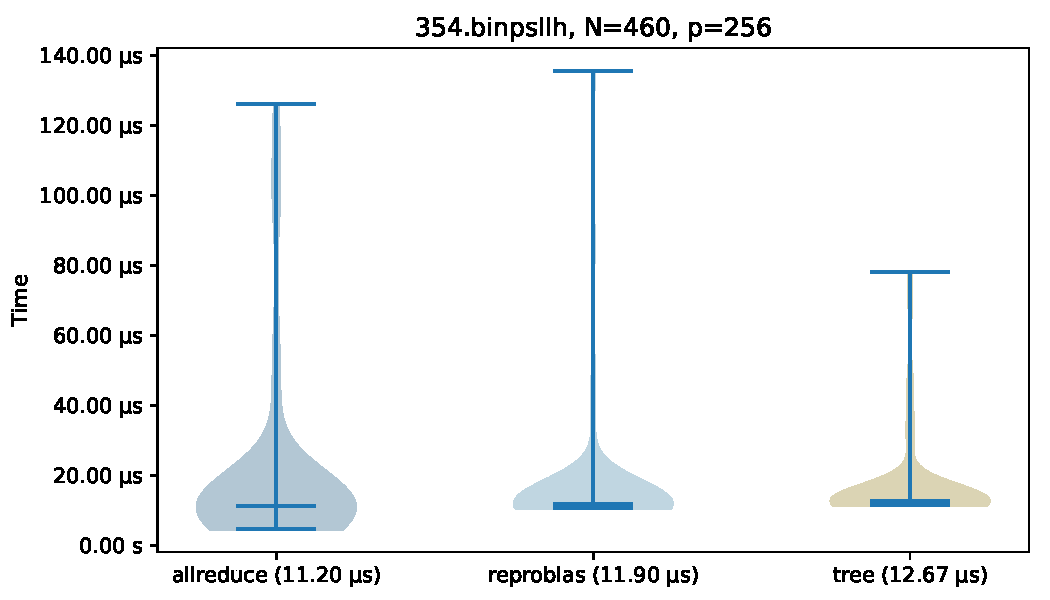
\includegraphics[scale=\mScale]{figures/violin354.pdf}
\end{subfigure}

\begin{subfigure}{\textwidth}
\centering
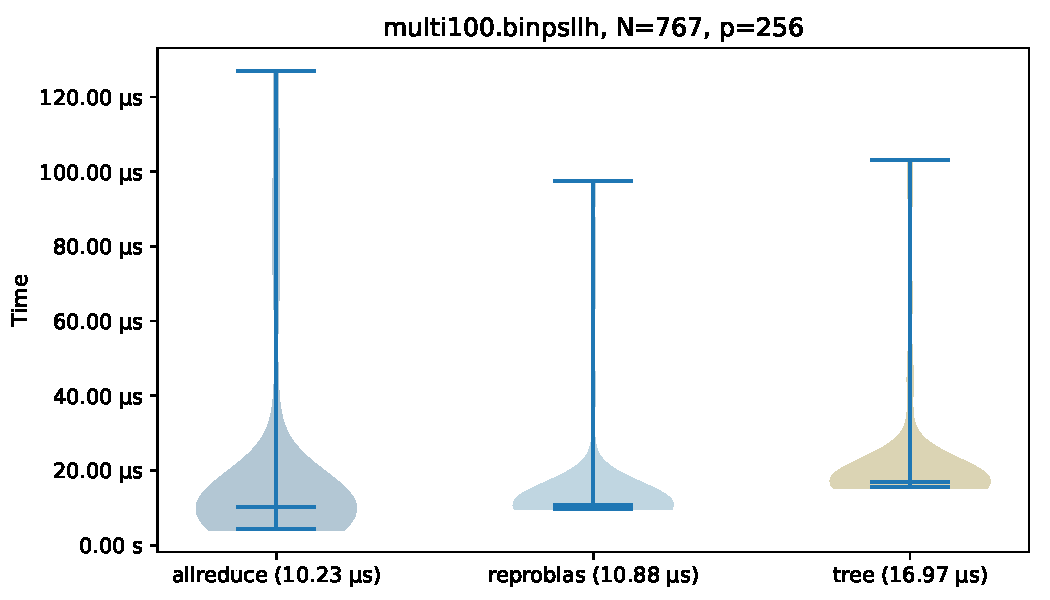
\includegraphics[scale=\mScale]{figures/violinMulti100.pdf}
\end{subfigure}

\begin{subfigure}{\textwidth}
\centering
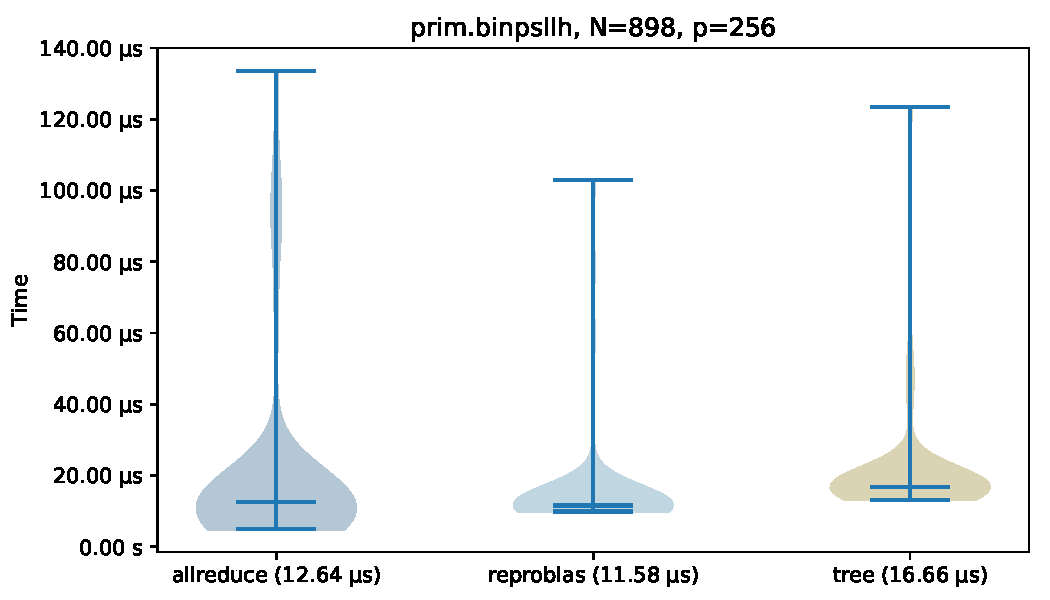
\includegraphics[scale=\mScale]{figures/violinPrim.pdf}
\end{subfigure}


\end{figure}
\begin{figure}\centering\ContinuedFloat

\begin{subfigure}{\textwidth}
\centering
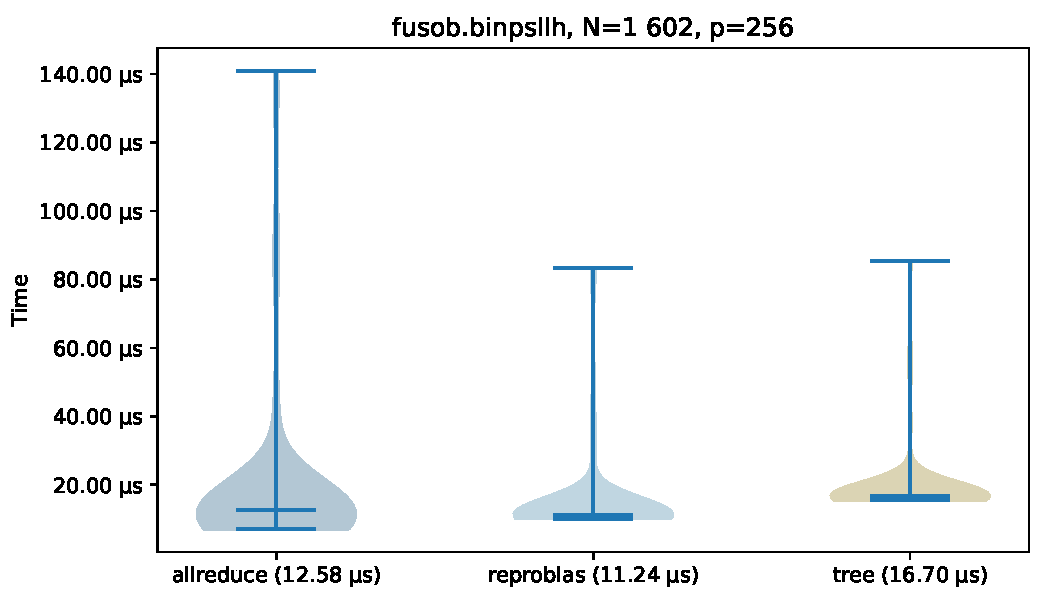
\includegraphics[scale=\mScale]{figures/violinFusob.pdf}
\end{subfigure}

\begin{subfigure}{\textwidth}
\centering
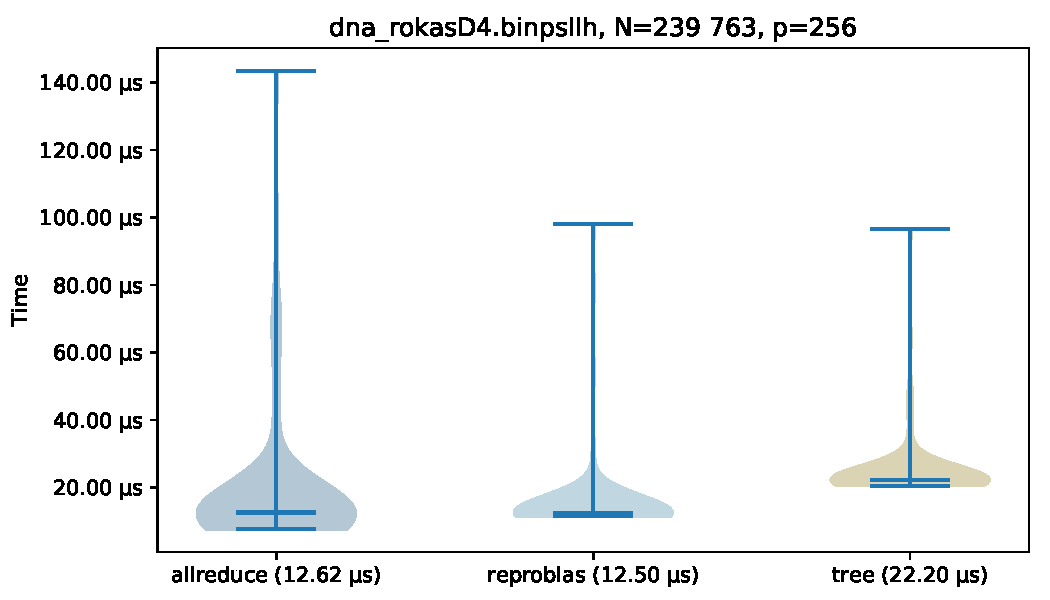
\includegraphics[scale=\mScale]{figures/violinRokasD4.pdf}
\end{subfigure}

\begin{subfigure}{\textwidth}
\centering
\includegraphics[scale=\mScale]{figures/violinRokasA8.pdf}
\end{subfigure}

\end{figure}
\begin{figure}\centering\ContinuedFloat

\begin{subfigure}{\textwidth}
\centering
\includegraphics[scale=\mScale]{figures/violinRokasD1.pdf}
\end{subfigure}


\begin{subfigure}{\textwidth}
\centering
\includegraphics[scale=\mScale]{figures/violinRokasA4.pdf}
\end{subfigure}

\begin{subfigure}{\textwidth}
\centering
\includegraphics[scale=\mScale]{figures/violinPeteD8.pdf}
\end{subfigure}

\end{figure}
\begin{figure}\centering\ContinuedFloat


\begin{subfigure}{\textwidth}
\centering
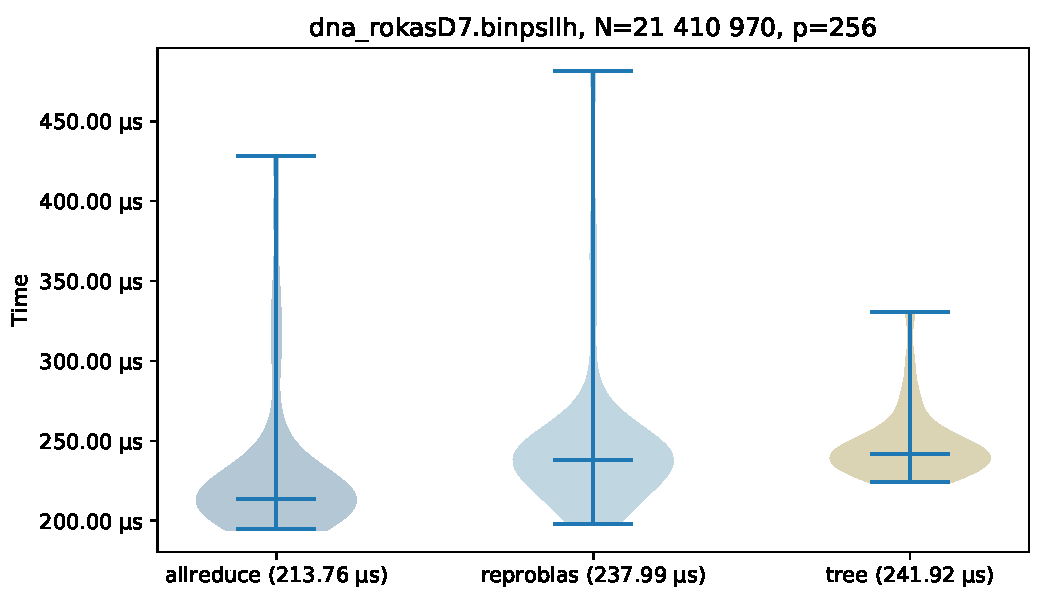
\includegraphics[scale=\mScale]{figures/violinRokasD7.pdf}
\end{subfigure}

\caption{Runtime distribution for all datasets with $p=256$ \glspl{pe}.}

\end{figure}

\begin{figure}
\centering
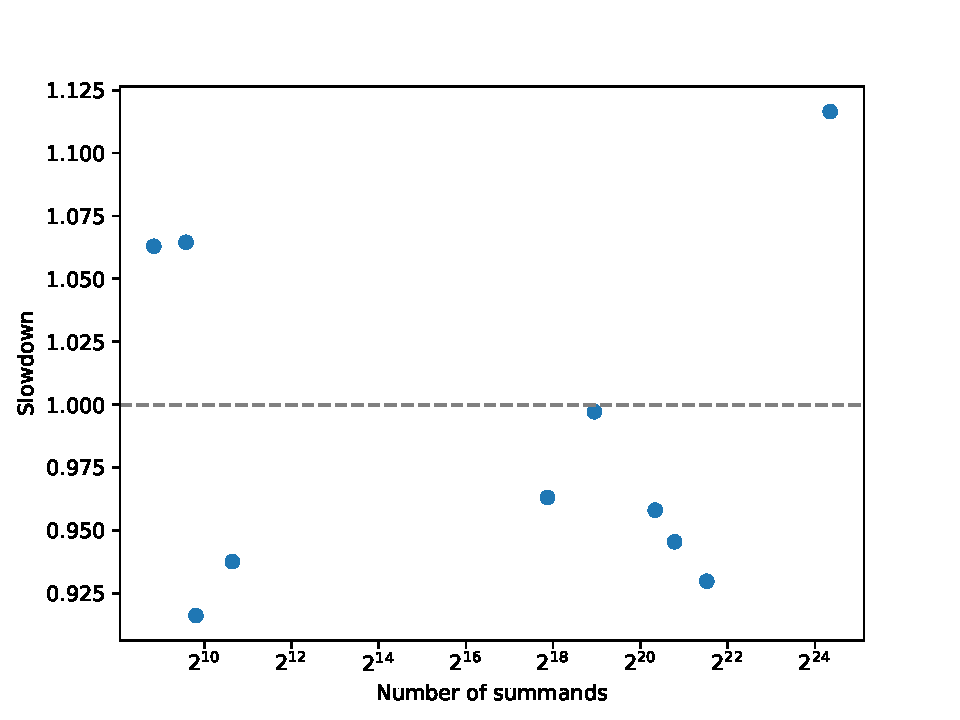
\includegraphics[scale=\mScale]{figures/slowdownAllreduceReproblas.pdf}
\caption{Slowdown of ReproBLAS compared to Allreduce ($p = 256$).}
\label{fig:slowdownAllreduceReproblas}
\end{figure}

\begin{figure}
\centering
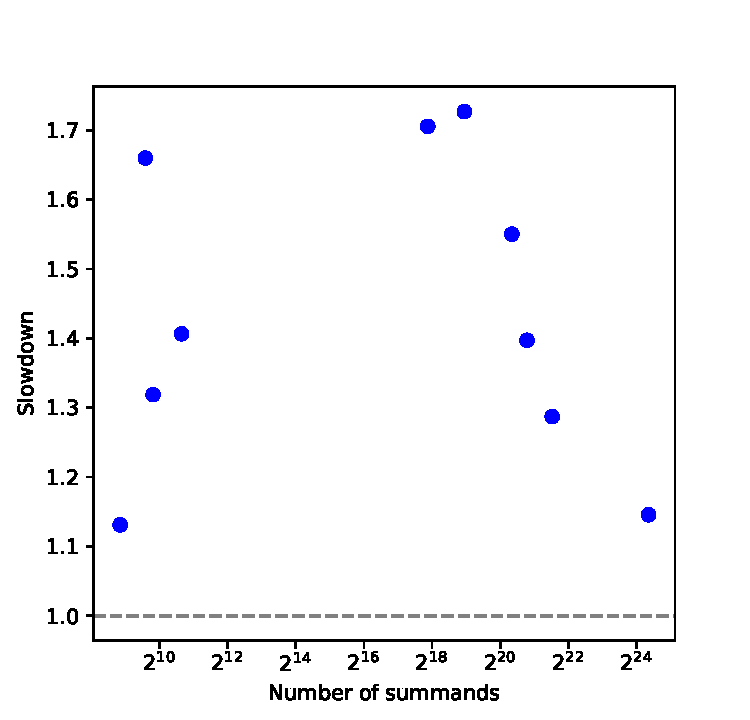
\includegraphics[scale=\mScale]{figures/slowdownAllreduceTree.pdf}
\caption{Slowdown of Binary Tree Summation compared to Allreduce ($p = 256$).}
\label{fig:slowdownAllreduceTree}
\end{figure}

\newpage
\section{Message Count Maxima}

\begin{figure}[H]
\centering
% N = 16, p = 4
\begin{subfigure}{1.0\textwidth}
\begin{tikzpicture}
\newcommand{\heightFactor}{0.7}
\newcommand{\treeN}{15}
\newcommand{\subtreeHeight}[2]{\directlua{tex.write(subtree_height(#1,#2))}}
\newcommand{\parentIdx}[1]{\directlua{tex.write(parent(#1))}}
\foreach \x in {0,1,...,\treeN} {
	\node [anchor=south] (idx\x) at (\x,0) {\x};

	
	\draw (\x,0)
		-- (\x,-\heightFactor * \subtreeHeight{\x}{\treeN}-\heightFactor)
		-- (\parentIdx{\x},-\heightFactor * \subtreeHeight{\x}{\treeN}-\heightFactor);
}

\draw [very thick, dashed, rounded corners, teal] (-0.5,0.5)  rectangle (3.4,-4.5 * \heightFactor);
\draw [very thick, dashed, rounded corners, olive]  (3.6, 0.5) rectangle (7.4,-3.5 * \heightFactor);
\draw [very thick, dashed, rounded corners, teal]  (7.6, 0.5) rectangle (11.4,-4.5 * \heightFactor);
\draw [very thick, dashed, rounded corners, olive]  (11.6, 0.5) rectangle (15.4,-3.5 * \heightFactor);

\foreach \x in {0,1,2,3}
\node (PE\x) at (1.5+4*\x,1) {\gls{pe} \x};
\end{tikzpicture}

\caption{Optimal distribution of $N=2^2*p$ elements over $p=4$ \glspl{pe}.}
\label{fig:messageCountShiftingOptimal}
\end{subfigure}

% N = 17, p = 4
\begin{subfigure}{1.0\textwidth}
\begin{tikzpicture}
\newcommand{\heightFactor}{0.7}
\newcommand{\treeN}{16}
\newcommand{\subtreeHeight}[2]{\directlua{tex.write(subtree_height(#1,#2))}}
\newcommand{\parentIdx}[1]{\directlua{tex.write(parent(#1))}}
\foreach \x in {0,1,...,\treeN} {
	\node [anchor=south] (idx\x) at (\x,0) {\x};

	
	\draw (\x,0)
		-- (\x,-\heightFactor * \subtreeHeight{\x}{\treeN}-\heightFactor)
		-- (\parentIdx{\x},-\heightFactor * \subtreeHeight{\x}{\treeN}-\heightFactor);
}

\draw [very thick, dashed, rounded corners, teal] (-0.5,0.5)  rectangle (4.4,-5.5 * \heightFactor);
\draw [very thick, dashed, rounded corners, olive]  (4.6, 0.5) rectangle (8.4,-4.5 * \heightFactor);
\draw [very thick, dashed, rounded corners, teal]  (8.6, 0.5) rectangle (12.4,-3.5 * \heightFactor);
\draw [very thick, dashed, rounded corners, olive]  (12.6, 0.5) rectangle (16.4,-5.5 * \heightFactor);

\node (PE0) at (2,1) {\gls{pe} 0};

\foreach \x in {1,2,3}
\node (PE\x) at (2.5+4*\x,1) {\gls{pe} \x};
\end{tikzpicture}
\caption{Worst-case distribution of $N=2^2*p+1$ elements over $p=4$ \glspl{pe}.}
\label{fig:messageCountShiftingWorstCase}
\end{subfigure}

\caption{Illustration of the shifting behaviour in the $n_i^\textrm{lower}$-distribution that produces maximal message counts.}
\label{fig:messageCountShifting}
\end{figure}

